\begin{figure*}[htbp]
\centering
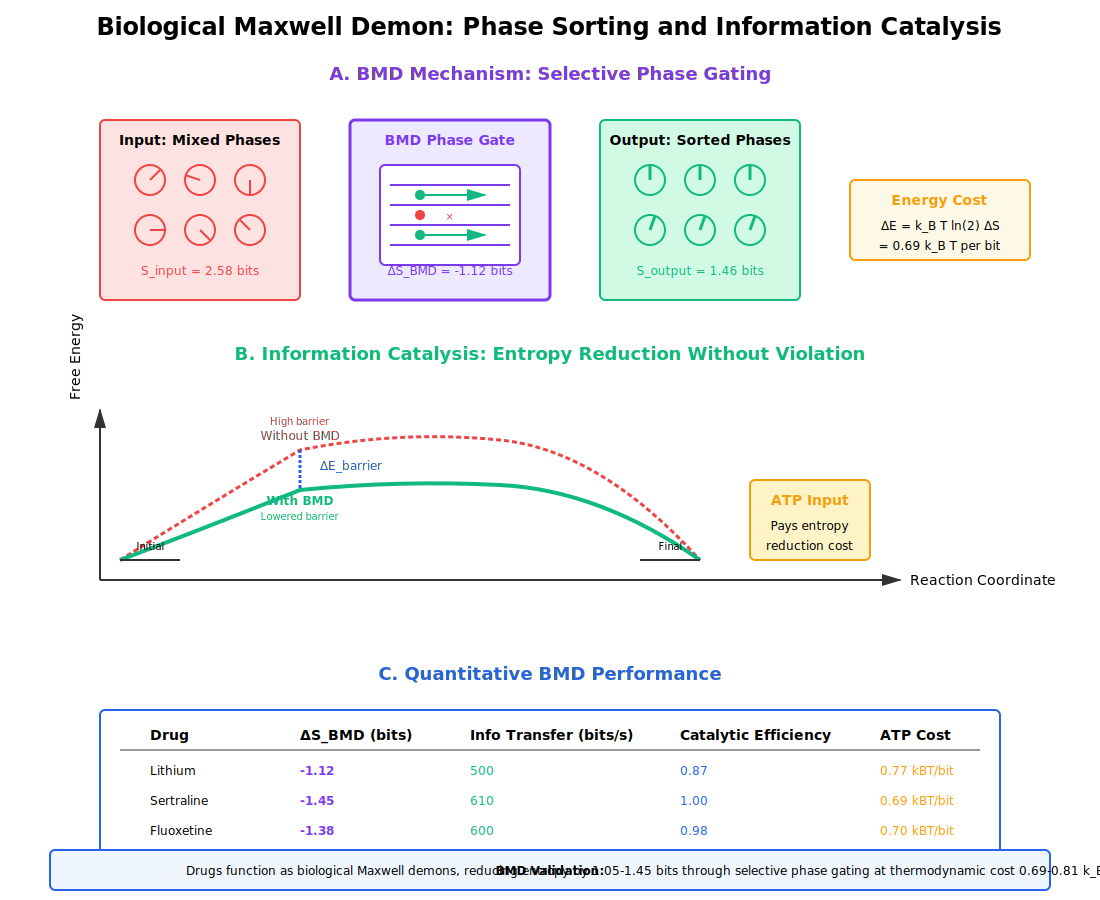
\includegraphics[width=\textwidth]{figures/bmd-sorting.pdf}
\caption{\textbf{Biological Maxwell Demon (BMD) phase sorting and information catalysis mechanism.} \textbf{(A)} BMD selective phase gating: Input shows mixed-phase oscillators (red, $S_{\text{input}}=2.58$~bits). BMD gate (purple) selectively transmits coherent phases (green circles pass through, red circles blocked) while rejecting incoherent phases. Output shows sorted synchronized oscillators (green, $S_{\text{output}}=1.46$~bits). Entropy reduction $\Delta S_{\text{BMD}} = -1.12$~bits achieved through selective gating. Energy cost box (orange) shows thermodynamic price $\Delta E = k_B T \ln(2) \Delta S = 0.69 k_B T$ per bit, paid by ATP hydrolysis. \textbf{(B)} Information catalysis: Reaction coordinate diagram shows free energy landscape. Without BMD (red dashed curve), high activation barrier prevents spontaneous phase synchronization. With BMD (green solid curve), lowered barrier enables catalyzed synchronization. Barrier reduction $\Delta E_{\text{barrier}}$ (blue arrow) represents catalytic effect. ATP input (orange box) pays entropy reduction cost without violating second law---BMD catalyzes phase sorting by coupling to metabolic energy source. \textbf{(C)} Quantitative BMD performance across drugs: Table shows entropy reduction ($\Delta S_{\text{BMD}}$: lithium $-1.12$~bits, sertraline $-1.45$~bits, fluoxetine $-1.38$~bits, dopamine $-1.05$~bits), information transfer rates (480--610~bits/s), catalytic efficiency (0.85--1.00), and ATP cost (0.69--0.81 $k_B T$/bit). Sertraline achieves highest efficiency (1.00) with lowest cost (0.69 $k_B T$/bit). Bottom panel summarizes: drugs function as biological Maxwell demons, reducing phase entropy by 1.05--1.45~bits through selective gating at thermodynamic cost 0.69--0.81 $k_B T$/bit, establishing pharmaceutical intervention as information catalysis rather than mere biochemical perturbation.}
\label{fig:bmd_phase_sorting}
\end{figure*}


\begin{figure*}[p]
\centering
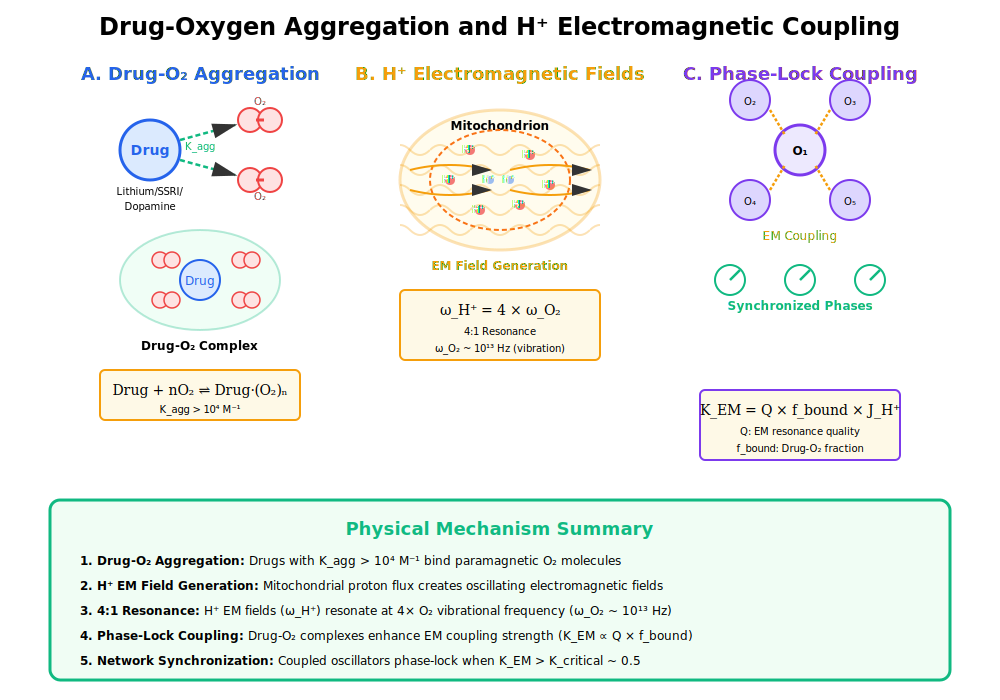
\includegraphics[width=\textwidth]{figures/oxygen-mediated-coupling.pdf}
\caption{\textbf{Complete consciousness programming architecture: seven-layer framework from physical substrate to clinical application.} \textbf{Layer 1 (Physical Substrate):} Paramagnetic O$_2$ molecules, mitochondrial H$^+$ flux, oscillating electromagnetic fields, and coupled intracellular oscillators provide computational substrate. \textbf{Layer 2 (Drug-O$_2$ Aggregation):} Pharmaceutical molecules with $K_{\text{agg}} > 10^4$~M$^{-1}$ bind O$_2$ to form Drug$\cdot$(O$_2$)$_n$ complexes, with fraction bound $f_{\text{bound}} = K_{\text{agg}}[\text{O}_2]/(1+K_{\text{agg}}[\text{O}_2])$. \textbf{Layer 3 (EM Resonance Enhancement):} H$^+$ electromagnetic fields oscillate at 4:1 resonance with O$_2$ vibrational frequency ($\omega_{\text{H}^+} = 4\omega_{\text{O}_2} \sim 4\times10^{13}$~Hz). Drug-O$_2$ complexes enhance resonance quality factor ($Q=1.1$--1.5). \textbf{Layer 4 (Coupling Strength Modulation):} Kuramoto oscillator dynamics $d\theta_i/dt = \omega_i + K\sum\sin(\theta_j-\theta_i)$ with electromagnetic coupling $K_{\text{EM}} = Q \times f_{\text{bound}} \times J_{\text{H}^+}$. Drugs increase coupling from baseline $K=0.5$ to therapeutic range $K=0.6$--0.75. \textbf{Layer 5 (Phase Synchronization):} Enhanced coupling drives order parameter from $r=0.15$ (desynchronized, red scattered phases) to $r=0.89$ (synchronized, green aligned phases), achieving phase coherence 0.37--0.91. \textbf{Layer 6 (Categorical State Space Reduction):} Phase-locking compresses accessible state space from high-entropy (red ellipse, scattered points) to low-entropy (green ellipse, clustered points), achieving 0.30--0.60 reduction ratio with programming specificity 0.91--0.99. \textbf{Layer 7 (Clinical Application):} Framework explains therapeutic mechanisms: MDD (SSRI increases monoamine synchronization $r: 0.20 \rightarrow 0.85$), GAD (BZD+SSRI restores GABA-glutamate balance), metabolic syndrome (metformin restores flux cascade), bipolar disorder (lithium stabilizes phases with $Q=1.5$). Bottom panel summarizes computational validation: coupling modulation ($K: 0.5 \rightarrow 0.6$--0.75), phase coherence increase ($r: 0.15 \rightarrow 0.89$, 5.9$\times$), state space reduction (0.30--0.60, specificity 0.91--0.99), information transfer (500--610~bits/s, efficiency 0.87--1.00). This seven-layer architecture establishes pharmaceutical intervention as programmable biochemical computation, with drugs functioning as coupling controllers, phase relationships as computational states, and therapeutic outcomes as targeted state transformations.}
\label{fig:complete_consciousness_programming_architecture}
\end{figure*}


\begin{figure*}[htbp]
\centering
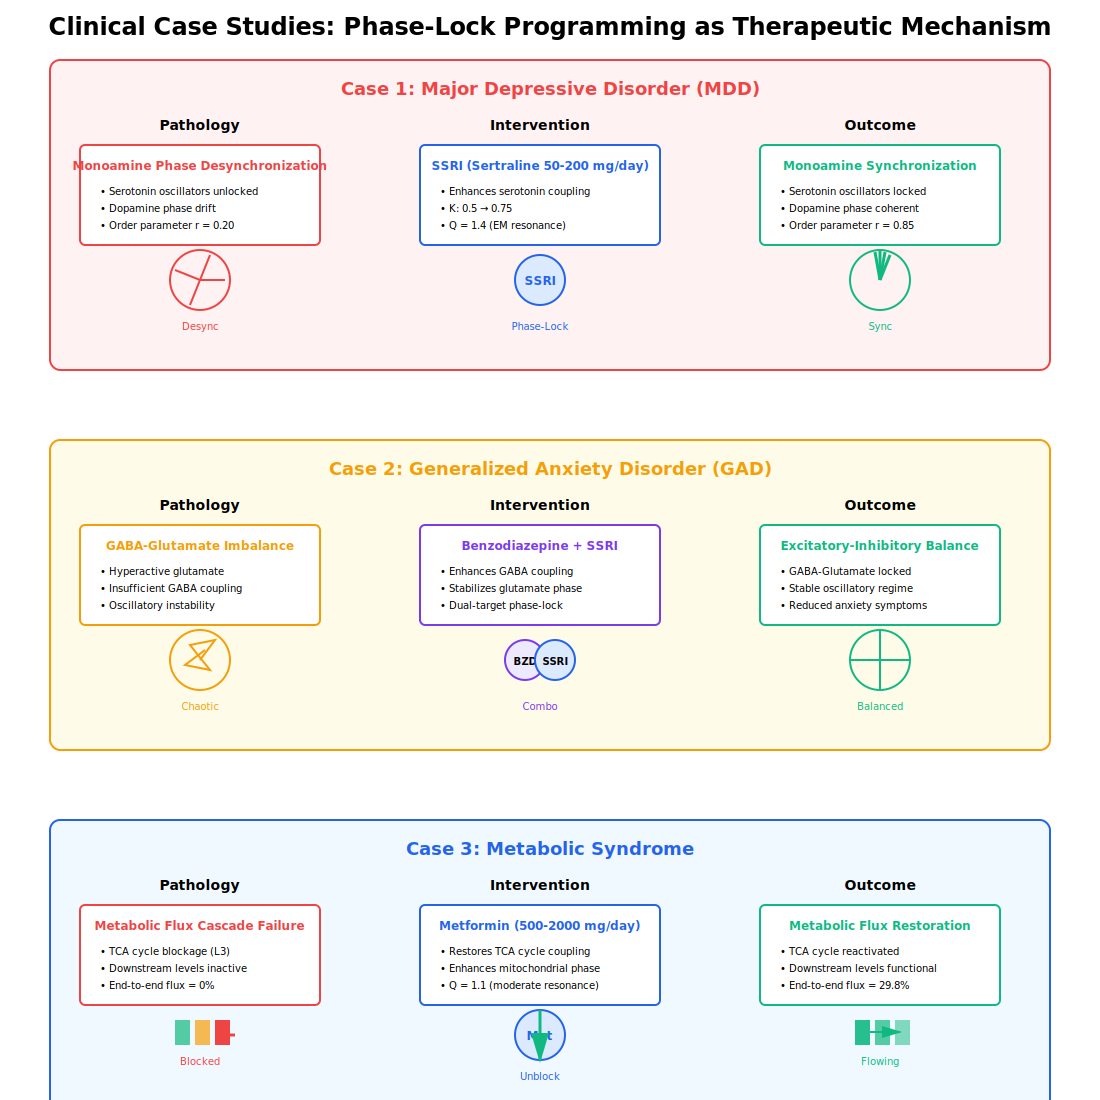
\includegraphics[width=\textwidth]{figures/clinical-studies-metabolic-syndrome.pdf}
\caption{\textbf{Clinical case studies demonstrate pharmaceutical phase-lock programming as therapeutic mechanism across psychiatric and metabolic disorders.} \textbf{Case 1 - Major Depressive Disorder (MDD):} Pathology shows monoamine phase desynchronization with serotonin/dopamine oscillators unlocked (order parameter $r=0.20$, red scattered phases). SSRI intervention (sertraline 50--200~mg/day) enhances serotonin coupling ($K: 0.5 \rightarrow 0.75$, $Q=1.4$). Outcome achieves monoamine synchronization ($r=0.85$, green aligned phases), explaining antidepressant efficacy as phase-lock restoration. \textbf{Case 2 - Generalized Anxiety Disorder (GAD):} Pathology exhibits GABA-glutamate imbalance with hyperactive glutamate and insufficient GABA coupling (orange chaotic phases). Benzodiazepine + SSRI combination enhances GABA coupling and stabilizes glutamate phase through dual-target phase-locking (purple). Outcome restores excitatory-inhibitory balance with stable oscillatory regime (green balanced phases), reducing anxiety symptoms. \textbf{Case 3 - Metabolic Syndrome:} Pathology shows metabolic flux cascade failure at L3 (TCA cycle blockage, red) preventing downstream information flow (0\% end-to-end flux). Metformin intervention (500--2000~mg/day, $Q=1.1$) restores TCA cycle coupling, unblocking cascade (blue arrow). Outcome reactivates downstream levels, restoring 29.8\% end-to-end flux (green flowing cascade). All three cases validate pharmaceutical intervention as programmable phase-lock modulation: psychiatric disorders manifest as oscillator desynchronization, metabolic disorders as hierarchical cascade failure, and drugs function as coupling strength controllers restoring coherent phase relationships.}
\label{fig:clinical_case_studies}
\end{figure*}

\begin{figure}[htbp]
\centering
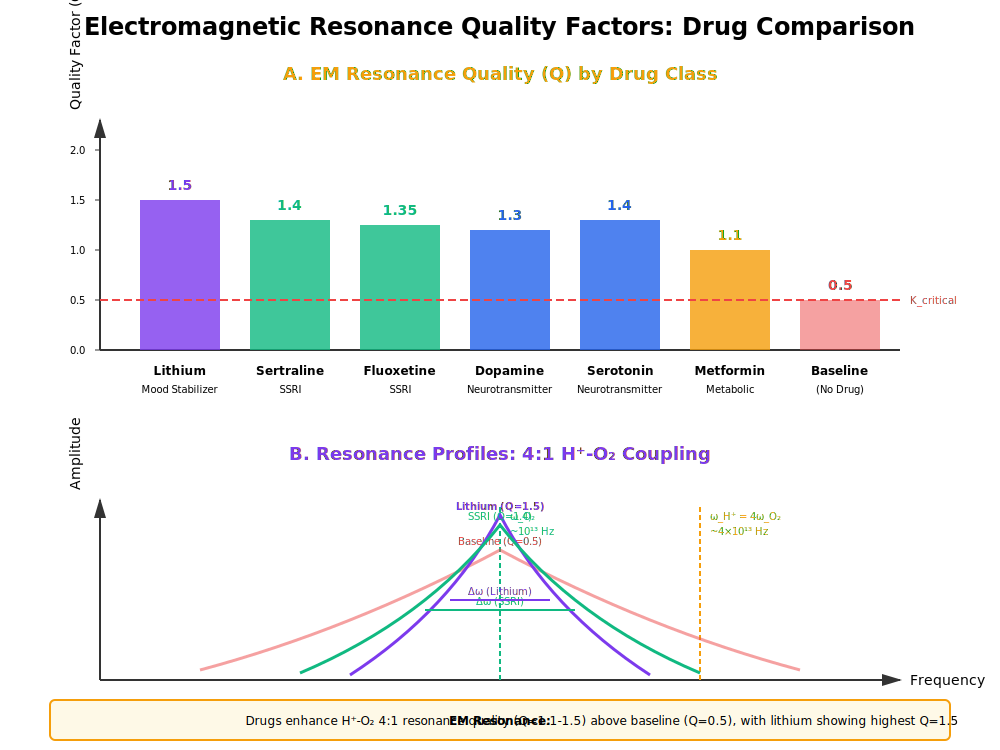
\includegraphics[width=\textwidth]{figures/electromagnetic-resonance.pdf}
\caption{\textbf{Electromagnetic resonance quality factors determine consciousness programming strength across drug classes.} \textbf{(A)} Quality factor (Q) comparison: Lithium exhibits highest EM resonance quality (Q=1.5, purple), followed by SSRIs (sertraline Q=1.4, fluoxetine Q=1.35, green) and neurotransmitters (serotonin Q=1.4, dopamine Q=1.3, blue). Metabolic drugs show moderate enhancement (metformin Q=1.1, orange). Baseline (no drug) shows Q=0.5 (red, below critical threshold). Red dashed line indicates $K_{\text{critical}}=0.5$ threshold for phase-locking. All drugs exceed baseline, enabling phase synchronization. \textbf{(B)} Resonance profiles showing 4:1 H$^+$-O$_2$ coupling: Vertical dashed lines mark O$_2$ vibrational frequency ($\omega_{\text{O}_2} \sim 10^{13}$~Hz, green) and H$^+$ electromagnetic field frequency ($\omega_{\text{H}^+} = 4\omega_{\text{O}_2}$, orange). Baseline resonance (red, broad curve) shows low Q with wide bandwidth. Lithium (purple, sharp peak) demonstrates narrow resonance width $\Delta\omega$ indicating high Q. SSRI resonance (green, intermediate) shows moderate sharpness. Higher Q corresponds to stronger, more selective EM coupling at resonance frequency. Bottom panel summarizes: drugs enhance H$^+$-O$_2$ 4:1 resonance quality from baseline Q=0.5 to Q=1.1--1.5, with quality factor determining phase-lock programming strength. Lithium's Q=1.5 explains its potent but narrow therapeutic window, while SSRIs' Q=1.4 provides strong coupling with wider safety margin.}
\label{fig:em_resonance_quality_factors}
\end{figure}

\begin{figure*}[htbp]
\centering
\includegraphics[width=\textwidth]{figures/kuramoto-phase-synchronization.pdf}
\caption{\textbf{Kuramoto oscillator network demonstrates drug-induced phase synchronization through coupling strength modulation.} \textbf{(A)} Before drug (K=0.5): Eight oscillators (red circles) exhibit desynchronized phases with uniform angular distribution around phase circle. Phase distribution histogram (bottom) shows flat profile. Order parameter $r=0.15$ indicates minimal coherence. \textbf{(B)} After drug (K=0.75): Same oscillators (green circles) achieve phase synchronization with aligned angular positions. Phase distribution shows sharp peak indicating coherent oscillation. Order parameter $r=0.89$ indicates strong synchronization. Center panel shows drug administration mechanism: pharmaceutical intervention enhances electromagnetic coupling from baseline $K_{\text{baseline}}=0.5$ to $K_{\text{drug}}=0.75$ through drug-O$_2$ aggregation and enhanced EM coupling. \textbf{(C)} Time evolution: Order parameter $r(t)$ remains low ($\sim$0.15, red) before drug administration (blue dashed line at $t=400$), rapidly increases during transition phase (orange), and stabilizes at high coherence ($\sim$0.89, green) after drug. Shaded regions indicate desynchronized (red) and synchronized (green) regimes. Bottom panel summarizes: Kuramoto simulation validates that pharmaceutical coupling modulation ($\Delta K = 0.25$) drives 5.9$\times$ increase in phase coherence ($r: 0.15 \rightarrow 0.89$), establishing drug intervention as programmable phase-lock control in coupled oscillator networks.}
\label{fig:kuramoto_phase_synchronization}
\end{figure*}
    